\documentclass[tikz]{standalone}
\usetikzlibrary{positioning}

\begin{document}
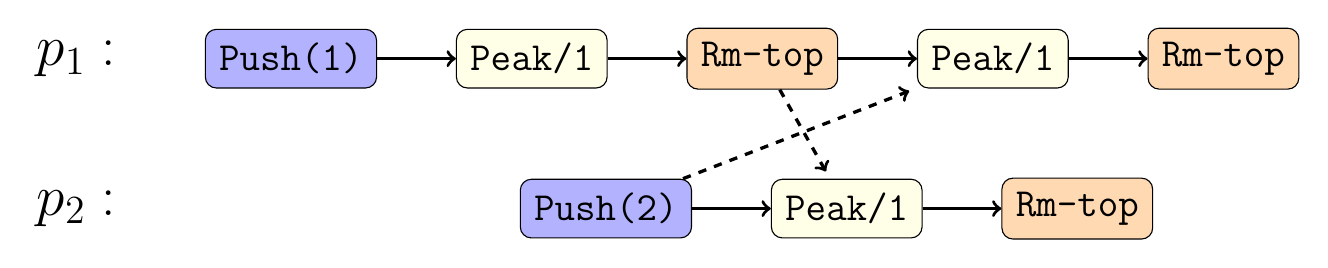
\begin{tikzpicture}
\tikzset{
  push-op/.style = {rectangle, rounded corners, fill = blue!30, draw, font = \Large, inner sep = 5pt},
  pop-peak/.style = {rectangle, rounded corners, fill = yellow!10, draw, font = \Large, inner sep = 5pt}, process/.style = {font = \huge}, po/.style = {->, very thick},
  pop-rt/.style = {rectangle, rounded corners, fill = orange!30, draw, font = \Large, inner sep = 5pt}, process/.style = {font = \huge}, po/.style = {->, very thick},
  vis/.style = {->, shorten >= 3pt, very thick, dashed}
}

  \node (p1) [process] {$p_1:$};
  \node (p1-push1) [push-op, right = 1.0cm of p1] {\texttt{Push(1)}};
  \node (p1-pop1-peak) [pop-peak, right = 1.0cm of p1-push1] {\texttt{Peak/1}};
  \node (p1-pop1-rt) [pop-rt, right = 1.0cm of p1-pop1-peak] {\texttt{Rm-top}};
  \node (p1-pop1'-peak) [pop-peak, right = 1.0cm of p1-pop1-rt] {\texttt{Peak/1}};
  \node (p1-pop1'-rt) [pop-rt, right = 1.0cm of p1-pop1'-peak] {\texttt{Rm-top}};

  \node (p2) [process, below = 1.2cm of p1] {$p_2:$};
  \node (p2-push2) [push-op, right = 5cm of p2] {\texttt{Push(2)}};
  \node (p2-pop1-peak) [pop-peak, right = 1.0cm of p2-push2] {\texttt{Peak/1}};
  \node (p2-pop1-rt) [pop-rt, right = 1.0cm of p2-pop1-peak] {\texttt{Rm-top}};

  \draw [po] (p1-push1) to (p1-pop1-peak);
  \draw [po] (p1-pop1-peak) to (p1-pop1-rt);
  \draw [po] (p1-pop1-rt) to (p1-pop1'-peak);
  \draw [po] (p1-pop1'-peak) to (p1-pop1'-rt);
  \draw [po] (p2-push2) to (p2-pop1-peak);
  \draw [po] (p2-pop1-peak) to (p2-pop1-rt);

  \draw [vis] (p2-push2) to (p1-pop1'-peak);
  \draw [vis] (p1-pop1-rt) to (p2-pop1-peak);

  %\draw [rw] (wx1) to [out = 0, in = 100] (rx1p3);

%  \node (p1-serial) [font = \huge, below right = 2.0cm and 3.0cm of p3] {$p_1:$ \texttt{W(x)0, W(x)1, W(y)2, W(y)3}};

\end{tikzpicture}
\end{document}